\section{Estado del arte}

% OSNT
\begin{frame}{The Open Source Network Tester}
  \begin{itemize}
    \item\alert<+>{Sistema de captura y reproducción de código abierto}
    \item\alert<+>{Utiliza cuatro FPGAs}
    \begin{itemize}
      \item Mismo modelo que la empleada en este TFG
    \end{itemize}
    \item\alert<+>{Gestionadas desde una interfaz sobre el propio servidor}
    \item\alert<+>{Se han identificado algunos aspectos mejorables}
    \begin{itemize}
      \item Provee información exclusivamente de la FPGA
      \item Interfaz poco intuitiva
      \item Se maneja desde el propio servidor
    \end{itemize}
    \item\alert<+>{Otras aplicaciones consideradas}
    \begin{itemize}
      \item tcpdump/libpcap
      \item Wireshark
      \item Detect-Pro
    \end{itemize}
  \end{itemize}
\end{frame}

% OSNT - Interfaz
\begin{frame}{The Open Source Network Tester - Interfaz}
  \begin{figure}
    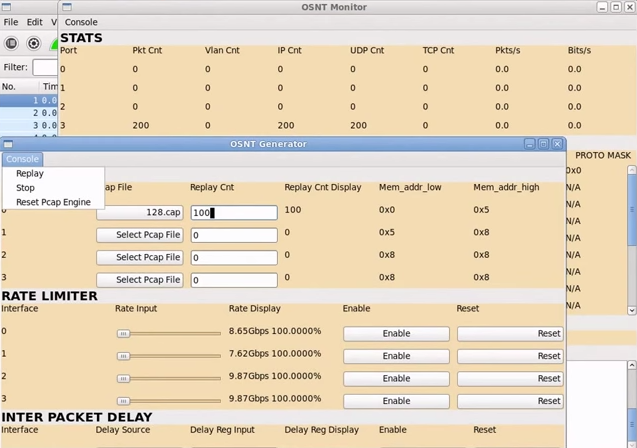
\includegraphics[width=0.9\linewidth]{osnt}
  \end{figure}
\end{frame}
